%---------------------------0-----------------------------------

\begin{frame}[c]{Geodengue}
  \begin{center}
      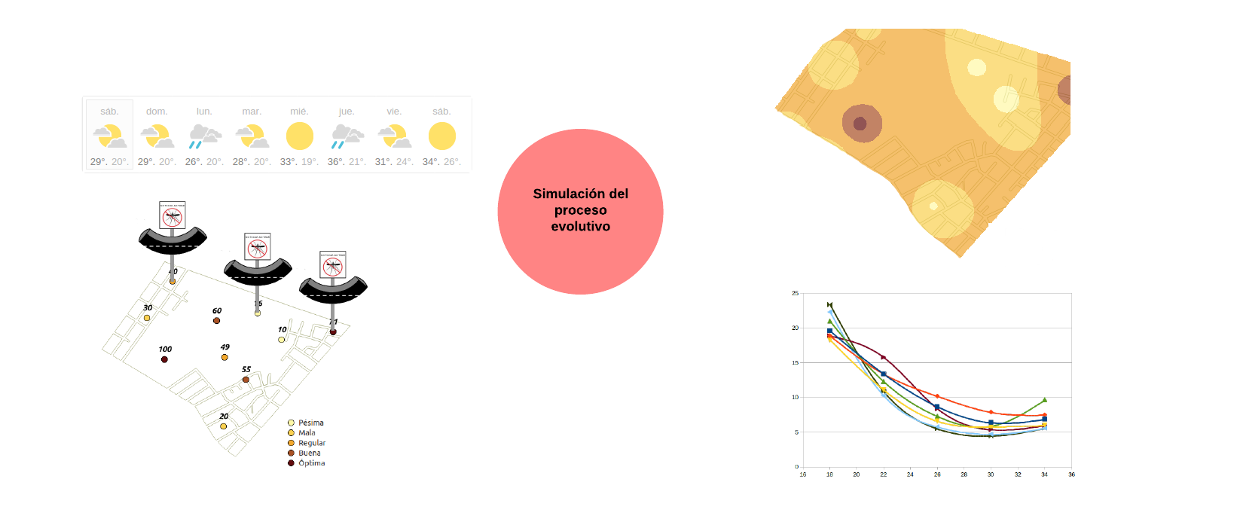
\includegraphics[width=\textwidth]{./graphics/propuesta.png}
  \end{center}
\end{frame}


%----------------------------2----------------------------------
\begin{frame}[c]{Preparación de datos de entrada}
  \begin{center}
    \begin{itemize}
      \item Selección del área de estudio.
      \item Distribución geográfica de los puntos de control.
      \item Revisión de los puntos de control.
      \item Generación de la población inicial a partir de los puntos de control.
      \item Obtener datos climáticos para el periodo de simulación.
    \end{itemize}
  \end{center}
\end{frame}
%-----------------------------3---------------------------------

\begin{frame}[c]{Preparación de datos de entrada. Conteo de larvas mediante PDI.}
Utilizar procesamiento digital de imágenes para agilizar el conteo de larvas obtenidas de las larvitrampas.
    \begin{figure}
      \begin{subfigure}[b]{0.4\textwidth}
          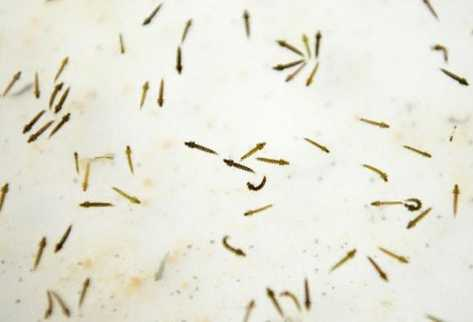
\includegraphics[width=\textwidth]{../book/capitulo-5/graphics/larvas-original.png}
          \caption{Imagen original antes de la transformación.}
      \end{subfigure}
      ~~~~
      \begin{subfigure}[b]{0.4\textwidth}
          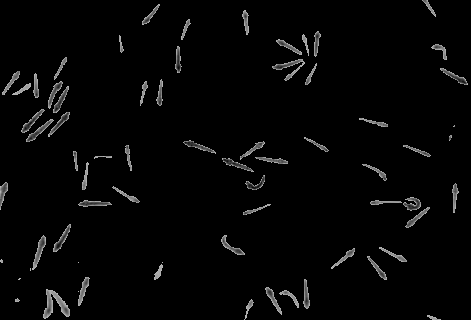
\includegraphics[width=\textwidth]{../book/capitulo-5/graphics/larvas-otsu.png}
          \caption{Imagen luego de la umbralización de Otsu.}
      \end{subfigure}
    \end{figure}
\end{frame}

%---------------------------4-----------------------------------

\begin{frame}[c]{Simulación del proceso evolutivo. Ciclo de vida del vector.}
  \begin{center}
      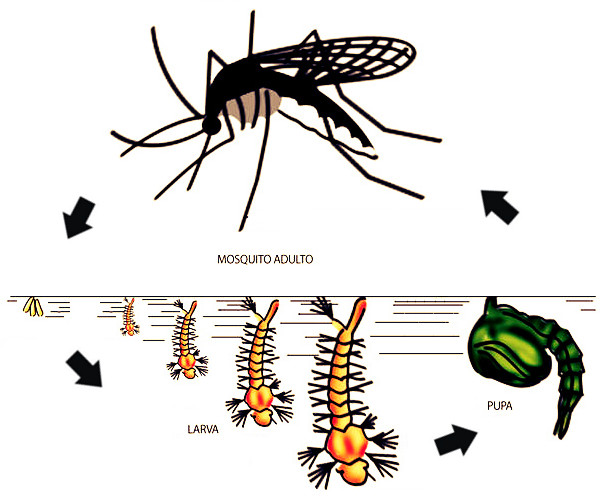
\includegraphics[width=7.8cm]{./graphics/ciclo-de-vida.jpg}
  \end{center}
\end{frame}


\begin{frame}[c]{Eventos que influyen en el ciclo de vida del vector.}
  \begin{itemize}
    \item Tasas de desarrollo para la eclosión de huevos, larvas, pupas y el ciclo gonotrófico de las hembras adultas.
    \item Mortalidad de huevos, larvas, pupas y mosquitos adultos.
    \item Dispersión de adultos.
    \item Ovipostura de hembras adultas nulíperas y paridas.
  \end{itemize}
\end{frame}

\begin{frame}[c]{Simulación del proceso evolutivo. Tasas de desarrollo}
  \begin{itemize}

    \item Las tasas dependen no sólo de valores de la población, sino también de la temperatura lo que introduce una dependencia del tiempo.

    \item El cálculo de las tasas de desarrollo se realiza mediante el modelo no lineal de Sharpe y DeMichele.

    \item El modelo debe ajustarse con los datos biológicos disponibles.
    \item El modelo puede utilizarse para calcular tasas de desarrollo a cualquier temperatura.
  \end{itemize}
\end{frame}


\begin{frame}[c]{Simulación del proceso evolutivo. Mortalidad}

\end{frame}


\begin{frame}[c]{Simulación del proceso evolutivo. Ciclo gonotrófico y Ovipostura.}
  \begin{center}
      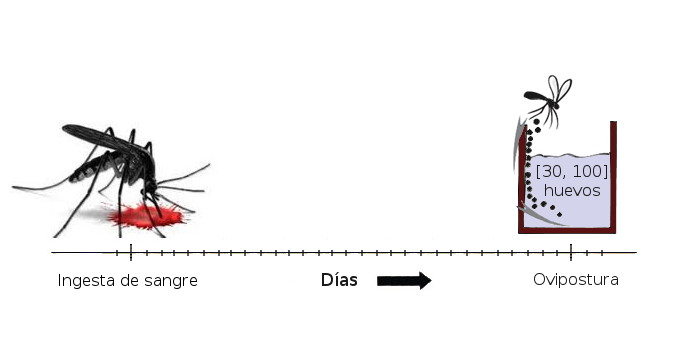
\includegraphics[width=\textwidth]{./graphics/cliclo-gonotrofico-tiempo.jpg}
  \end{center}
\end{frame}

\begin{frame}[c]{Simulación del proceso evolutivo. Dispersión.}
  \begin{center}
    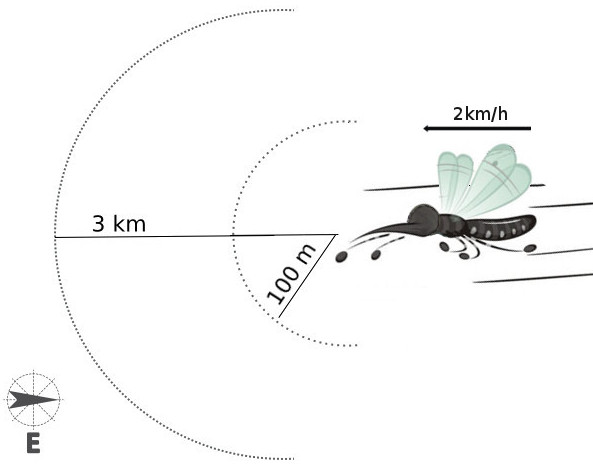
\includegraphics[width=8.5cm]{./graphics/dispersion.jpg}
  \end{center}
\end{frame}


\begin{frame}[c]{Simulación del proceso evolutivo}
  \begin{center}
    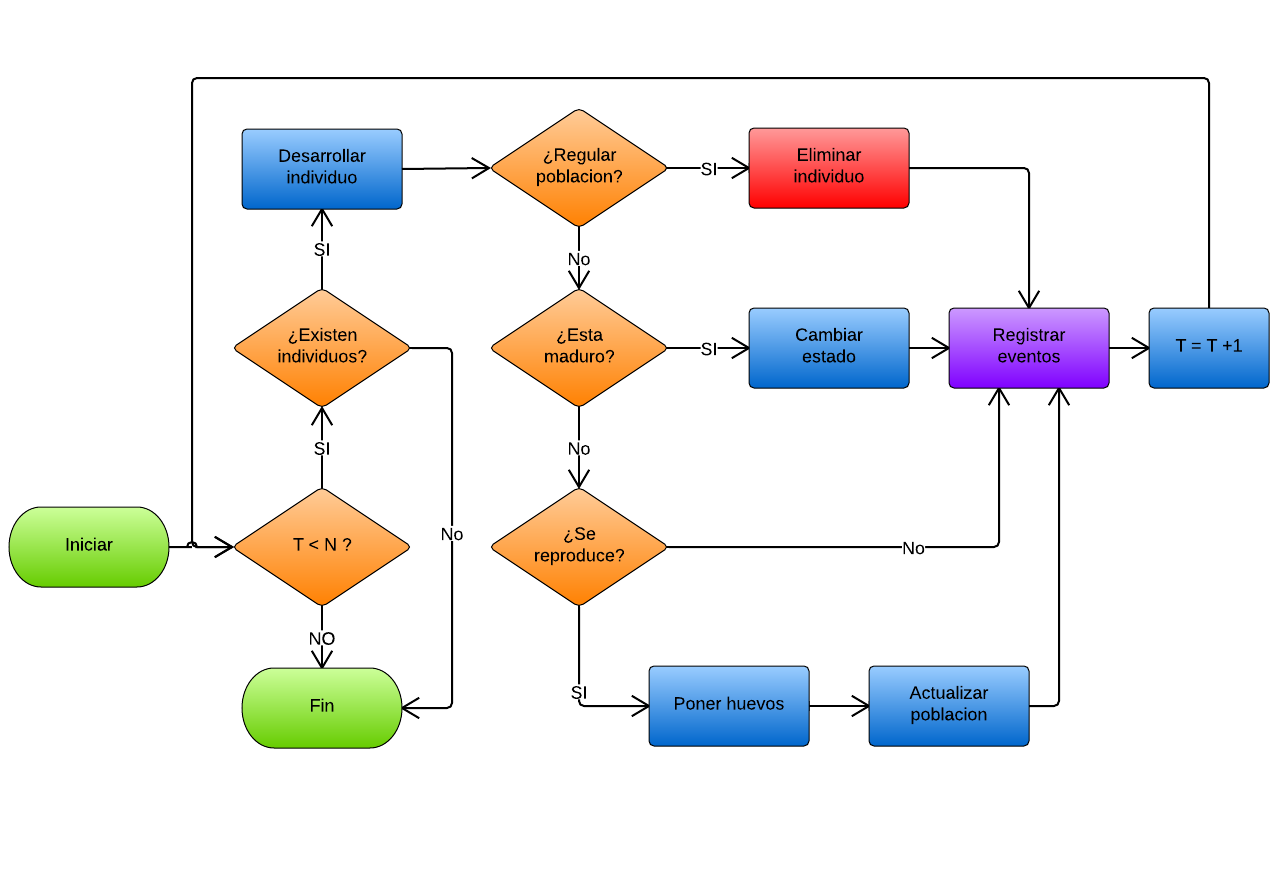
\includegraphics[height=7.5cm]{./graphics/algoritmo-propuesto.png}
  \end{center}
\end{frame}

%--------------------------5------------------------------------

\begin{frame}[c]{Clasificación de los niveles de infestación.}
  \begin{table}
    \begin{minipage}{\textwidth}
    \begin{center}
    \caption{\label{tab:cap4-puntaje-zona} Escala de clasificación de los niveles de infestación teniendo en cuenta la cantidad de larvas.}
      \begin{tabular}{l c c c c}
          \hline
                       &          &           & Hembras     & Hembras \\
          Tipo de zona &Mínimo$^a$& Máximo$^a$& Adultas$^b$ & Reproductivas $^c$\\
          \hline
          \hline
          Muy baja  & 0  & 19 & 8  & 5 \\
          Baja    & 20 & 35 & 15 & 10\\
          Normal & 36 & 51 & 22 & 15\\
          Alta   & 52 & 69 & 30 & 20\\
          Muy alta  & 70 & --$^d$  & --$^d$  & --$^d$ \\
      \end{tabular}
      \footnotetext[1]{Rango mínimo y máximo permitido el nivel.}
      \footnotetext[2]{Cantidad máxima de hembras adultas, al final del periodo de desarrollo.}
      \footnotetext[3]{Cantidad de hembras adultas con capacidad de oviponer.}
      \footnotetext[4]{No se estableció un límite superior para las niveles muy altos. }
      \end{center}
    \end{minipage}
  \end{table}
\end{frame}


\begin{frame}[t]{Clasificación de los niveles de infestación.}
  Consideraciones para la clasificación de los niveles de infestación:
  \begin{itemize}
      \item Solo el $50$ \% de las larvas observadas son hembras.
      \item La temperatura media anual es de 25 \textcelsius.
      \item La tasa mortalidad diaria natural de las larvas y pupas bajo optimas condiciones, a 25 \textcelsius, es igual a $0,01056$ 1/días respectivamente.
      \item La tasa de desarrollo, a 25 \textcelsius, de la larva hasta su emergencia a adulto es de $11,57$ días.
      \item El $32,10$ \% de las hembras adultas no oviponen.
  \end{itemize}
\end{frame}


\begin{frame}[c]{Análisis y presentación de los resultados}
  \begin{center}
      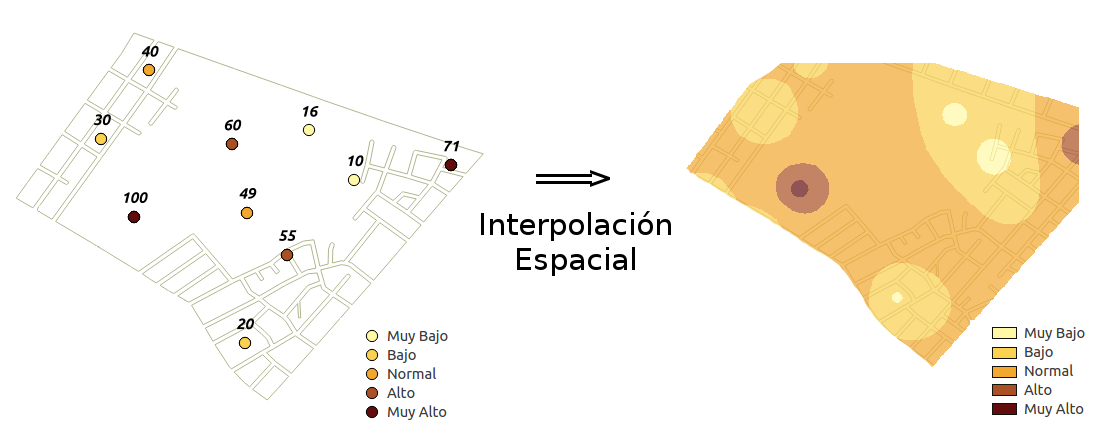
\includegraphics[width=\textwidth]{./graphics/identificacion-focos.png}
  \end{center}
\end{frame}

%--------------------------6------------------------------------

\begin{frame}[t]{Análisis y presentación de los resultados}
  \begin{center}
      \begin{itemize}
        \item Tasa promedio de desarrollo.
        \item Tasa promedio de mortalidad diaria.
        \item Cantidad promedio de huevos.
        \item Dispersión media.
        \item Cartografía del vector.
        \item Mapas de interpolación.
      \end{itemize}
  \end{center}
\end{frame}

